\chapter{System Implementation}  \label{Chapter:Implementation}


This chapter describes the internal details of my implementation of software project telemetry. The target audience is developers who wish to maintain and improve the telemetry core components. For developer who wants to implement additional telemetry reducers or end users, resources listed in Table \ref{table:Telemetry-User-Role-Resources} might be more useful.

\begin{table}[tbp]
	\centering
		\begin{tabular}{|p{0.35\textwidth}|p{0.40\textwidth}|p{0.15\textwidth}|} 
			\hline
			\textbf{Role} & \textbf{Resource} & \textbf{Link}\\
			
			\hline
			End User & Software Project Telemetry End User Guide; & Appendix \ref{Chapter:TelemetryUserGuide}\\
      {} & Software Project Telemetry Language Specification. & Appendix \ref{Chapter:TelemetryLanguageSpecification}\\
			          
			\hline
		  Telemetry Reducer Developer & Software Project Telemetry Reducer Developer Guide. & Appendix \ref{Chapter:TelemetryDeveloperGuide}\\
		 
			\hline
			Telemetry System Maintainer & System Implementation; & This Chapter\\
			{} & Software Project Telemetry Language Specification. & Appendix \ref{Chapter:TelemetryLanguageSpecification} \\
		
			\hline
		\end{tabular}
	\caption{Software Project Telemetry Resources}
	\label{table:Telemetry-User-Role-Resources}
\end{table}


The software project telemetry system is designed and implemented by me as part of my dissertation research. It is built on top of the Hackystat foundation leveraging its generic framework of metrics collection and project management. Hackystat is a framework that provides novel support for software measurement definition, validation, and software engineering experimentation. It is developed in Collaborative Software Development Lab (CSDL) at University of Hawaii. %and the general goal is to explore ways to provide software developers with automated support for collecting and analyzing interesting and useful measures of software development process and products. 

In a sense, the software project telemetry system can be viewed as an extension to the functionalities of the Hackystat framework. CSDL members sometimes use ``Hackystat'' as an umbrella term to refer to Hackystat infrastructure plus all extensions built on top of it. However, for the sake of clarity, this dissertation makes the distinction between Hackystat framework and the software project telemetry system. Throughout this dissertation:
\begin{itemize}
	\item \textit{Hackystat framework} --- refers to the infrastructure,
	\item \textit{Software project telemetry system} --- refers to my implementation of the telemetry concept utilizing that infrastructure.
\end{itemize}


The reason that I chose to base my implementation of software project telemetry on the Hackystat framework instead of building everything from scratch is because:

\begin{enumerate}
	\item Hackystat uses sensors to collect software metrics, which is an essential prerequisite for \textit{software project telemetry}. Its metrics collection subsystem is flexible, and new sensors can be easily plugged in.
	\item Hackystat offers sophisticated support for metrics data storage, processing, and presentation.
	\item Hackystat has flexible extension mechanism. New analyses and alerts can be easily plugged in.
%	\item Case studies in classroom settings indicated that Hackystat framework had very low overhead and Hackystat analyses are helpful \cite{Johnson:2003b} \cite{Johnson:2004}. 
	\item I have been on the development team of Hackystat since 2002 and have extensive knowledge of the framework.
\end{enumerate}







%%%%%%%%%%%%%%%%%%%%%%%%%%%%%%%%%%%%%%%%%%%%%%%%%%%%%%%%%
%                                                       %
%                   S E C T I O N                       %
%                                                       %
%%%%%%%%%%%%%%%%%%%%%%%%%%%%%%%%%%%%%%%%%%%%%%%%%%%%%%%%%

\section{Implementation Details}

The actual implementation details of software project telemetry are omitted in this proposal. Interested readers are encouraged to examine the following documents:
\begin{itemize}
	\item \textit{Telemetry Language Specification}:\\
	Appendix \ref{Chapter:TelemetryLanguageSpecification}
	
	\item \textit{Telemetry End User Documentation}:\\
	\special{html:<a href="http://hackystat.ics.hawaii.edu/hackystat/docbook/ch05.html">}
	http://hackystat.ics.hawaii.edu/hackystat/docbook/ch05.html 
	\special{html:</a>}
		
	\item \textit{Telemetry Developer Guide}:\\
	Appendix \ref{Chapter:TelemetryDeveloperGuide}

	\item \textit{Complete Source Code}:\\
	\special{html:<a href="http://hackydev.ics.hawaii.edu/hackyDevSite/lastBuild.do">}
	http://hackydev.ics.hawaii.edu/hackyDevSite/lastBuild.do
	\special{html:</a>}\\
	Please note that the source code is updated daily. Please follow the link ``Build Results'' -- ``java2html'', and the major portion of telemetry related implementation code is in the module ``hackyTelemetry''.
\end{itemize}


When the dissertation is complete, this chapter will be organized into the following sections. Section \ref{Chapter:Implementation}.\textcolor{red}{1} will give a brief introduction of Hackystat architecture. Section \ref{Chapter:Implementation}.\textcolor{red}{2} will detail \textit{software project telemetry} related implementation.



%%%%%%%%%%%%%%%%%%%%%%%%%%%%%%%%%%%%%%%%%%%%%%%%%%%%%%%%%
%                                                       %
%                   S E C T I O N                       %
%                                                       %
%%%%%%%%%%%%%%%%%%%%%%%%%%%%%%%%%%%%%%%%%%%%%%%%%%%%%%%%%

\section{Time Frame}

The implementation is complete. Two instances of the software project telemetry system are deployed. One is on the public Hackystat server which is used in the case studies in Chapter \ref{Chapter:EvaluationInClassroom} and \ref{Chapter:EvaluationInCSDL}. The other instance is deployed on Ikayzo server which is used in the case study in Chapter \ref{Chapter:EvaluationInIkayzo}.









%%%%%%%%%%%%%%%%%%%%%%%%%%%%%%%%%%%%%%%%%%%%%%%%%%%%%%%%%
%                                                       %
%   !!! Commented Out -- Everything below here !!!      %
%                                                       %
%%%%%%%%%%%%%%%%%%%%%%%%%%%%%%%%%%%%%%%%%%%%%%%%%%%%%%%%%

\begin{comment}


The reference implementation offers 3 interfaces to telemetry analysis.

\begin{itemize}
	\item Telemetry expert analysis - This is the most flexible interface. The use has the finest control from determining which software metrics to use, how to aggregate different metrics, to the display details of telemetry charts. In order to harness the power of the expert interface, the user has to learn telemetry language, as well as having a fairly deep understanding of how the system works. 
	
	\item Predefined telemetry chart analysis - A set of commonly used telemetry streams and charts are pre-configured by the instructor, and saved in the system. This relieves the user from learning the telemetry language. In order to use the interface, the user can simply ask the system for the predefined telemetry chart along with some chart-specific parameters. For example, one of the telemetry chart defined is source code size, which requires a parameter call file pattern to tell the system which files to be included in computation.
	
	\item Predefined telemetry report analysis - We grouped some telemetry charts together into telemetry reports to represent certain perspectives on software development, such as development progress, process stability, quality assurance progress, etc. 
\end{itemize}

During the course of the semester, the telemetry language has undergone several evolutions. As a result, telemetry language and the expert interface was not introduced in class. The students are taught how to use telemetry chart and report analysis interfaces, and they use these two interfaces to collect and analyze metrics while performing their software development tasks.




\subsection{Expert interface, normal interface, external daily reports}

In the current reference implementation of software project telemetry, there are 3 ways an end user can retrieve a telemetry chart. 

\begin{itemize}
	\item In expert mode, the user uses telemetry language to construct telemetry charts directly. The user has finest control from determining which software metrics to use, how to aggregate different metrics, to the display details of the chart. The flexibility comes at the cost of learning the telemetry language, knowing the types of metrics available to the system, as well as performing some one-time non-trial project related administrative configurations so that the system knows which metric belongs to which project. The expert mode enables a full experiential approach to project management - a user experiment with different telemetry charts and uncover relationships among metrics.
	
	\item In normal mode, the user does not have to know the telemetry language and retrieves predefined telemetry charts directly. The telemetry charts can be predefined either with the system distribution or by a software process expert who knows telemetry language. 
	
	\item Lastly, a set of scripts is offered so that predefined telemetry charts can be integrated in other systems and updated periodically. 
	
\end{itemize}


This saves ordinary user from learning a new language and lows adoption barrier at the cost of flexibility. There is a tradeoff to make. I will investigate which telemetry streams are frequently-invoked so that I can pre-define them and make them available in customized analysis by default. Custom-mode telemetry analysis invocation log can be analyzed to compute invocation count for each predefined telemetry stream or report. Expert-mode telemetry analysis invocation log can be used to find out new telemetry streams users are trying to generate. Based on above information, I can adjust pre-defined telemetry definitions.





















One of the main reason Hackystat is chosen: (1) it already uses sensors to collect metrics automatically and unobtrusively, (2) sophisticated metrics storage. I don't have to reinvent the wheel.  

In footnote: actually, my work on software project telemetry is inspired by Hackystat, and Hackystat predates software project telemetry.


This chapter is organized into the following sections. Section \ref{Implementation:Hackystat} gives a brief introduction of Hackystat architecture. Section \ref{Implementation:Telemetry} details \textit{software project telemetry} related implementation.






\section{Hackystat Framework}  \label{Implementation:Hackystat}

\begin{figure}[tbp]
  \centering
  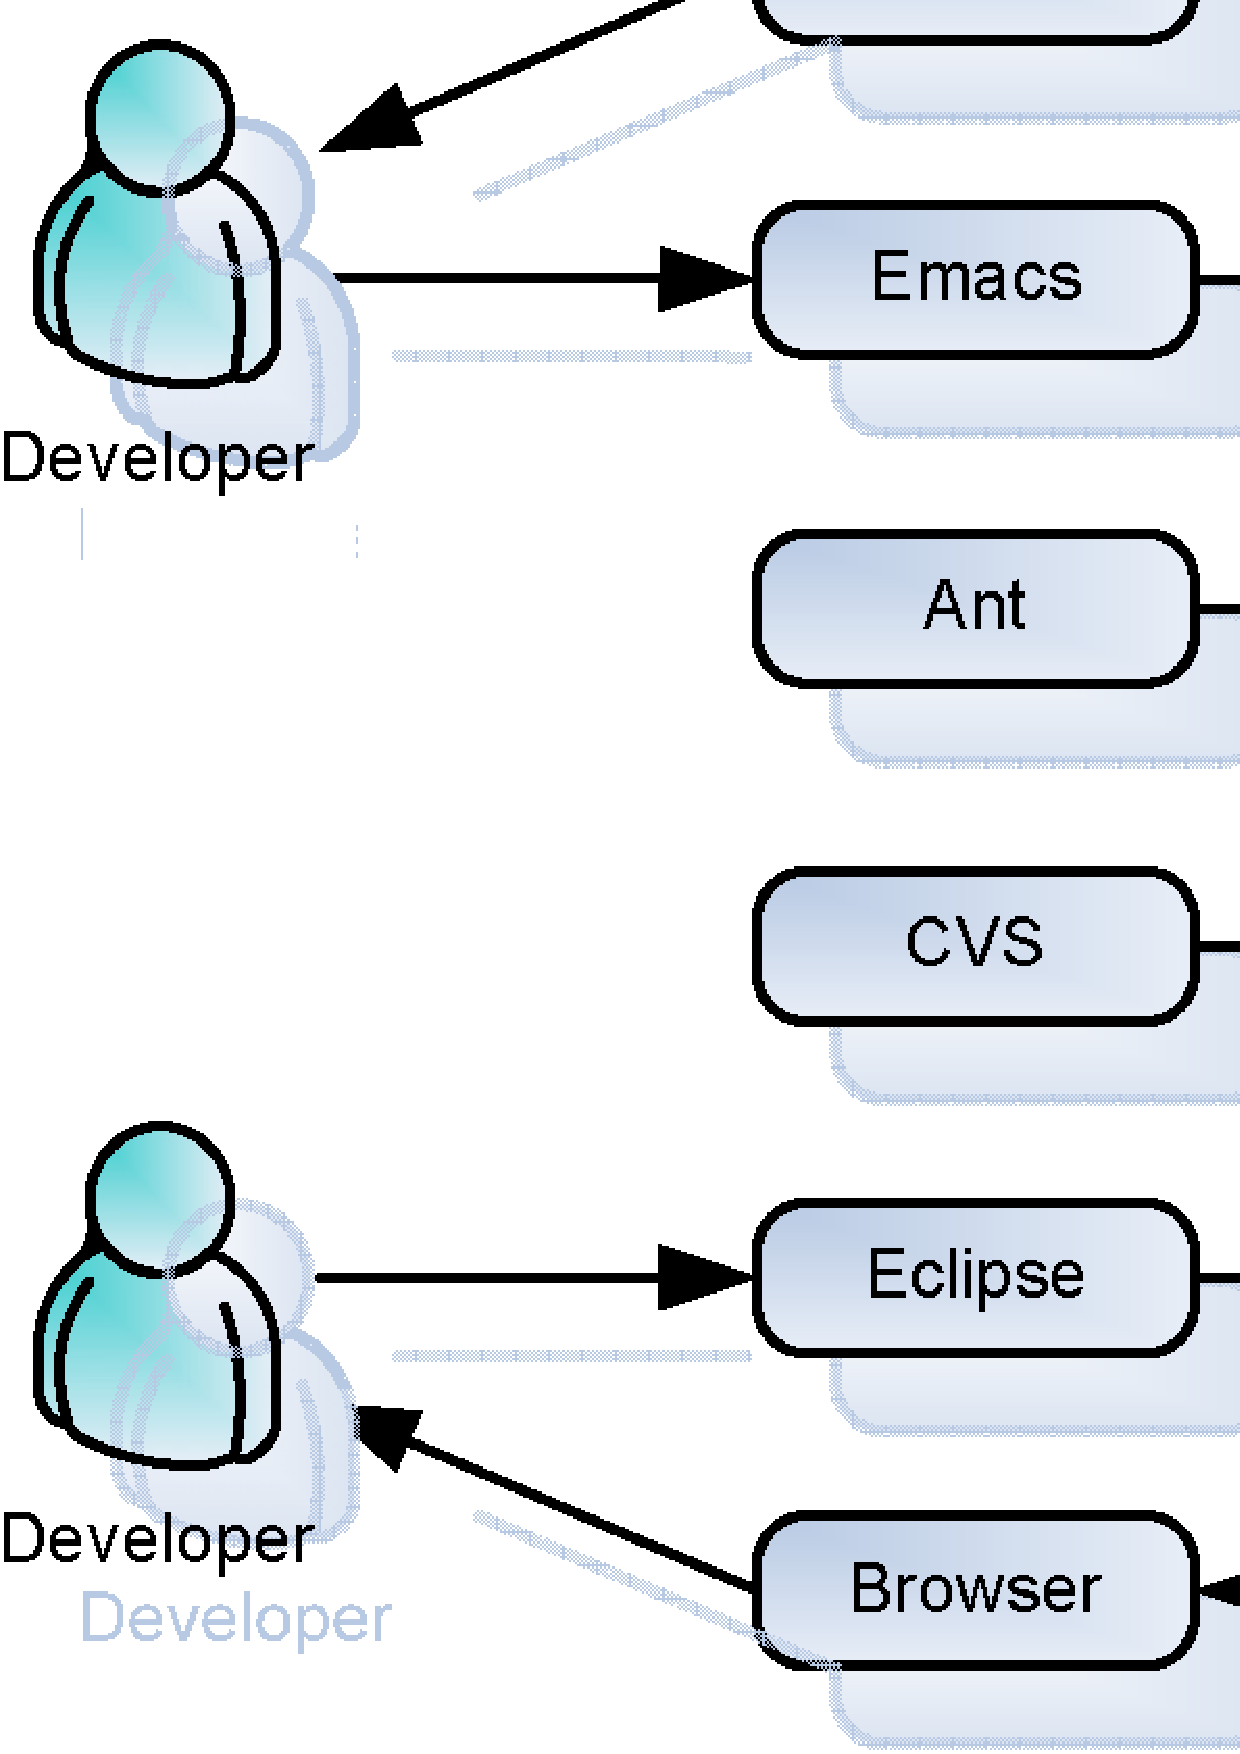
\includegraphics[width=1.00\textwidth]{figures/HackystatArchitecture}
  \caption{Hackystat Architecture - External View}
  \label{fig:HackystatArchitecture}
\end{figure}

The basic architecture of Hackystat is illustrated in Figure \ref{fig:HackystatArchitecture}. Software project development environment is instrumented by attaching sensors to various tools such as IDE, build system, configuration management system, and so forth. Once installed, sensors collect software process and product metrics automatically and unobtrusively, and send them to Hackystat server for storage and further processing. Developers can log onto the server through a web interface, and run analyses on their product and process metrics. Hackystat can send out automated alerts as well when incoming metrics activate user-defined triggers, such as the code the developer is editing exceeds some predefined threshold. 

Hackystat uses micro-kernel design. The kernel only provides essential services, such as receiving sensor data and managing their persistence. All analyses and alerts are implemented through through extensions.

\begin{figure}[tbp]
  \centering
  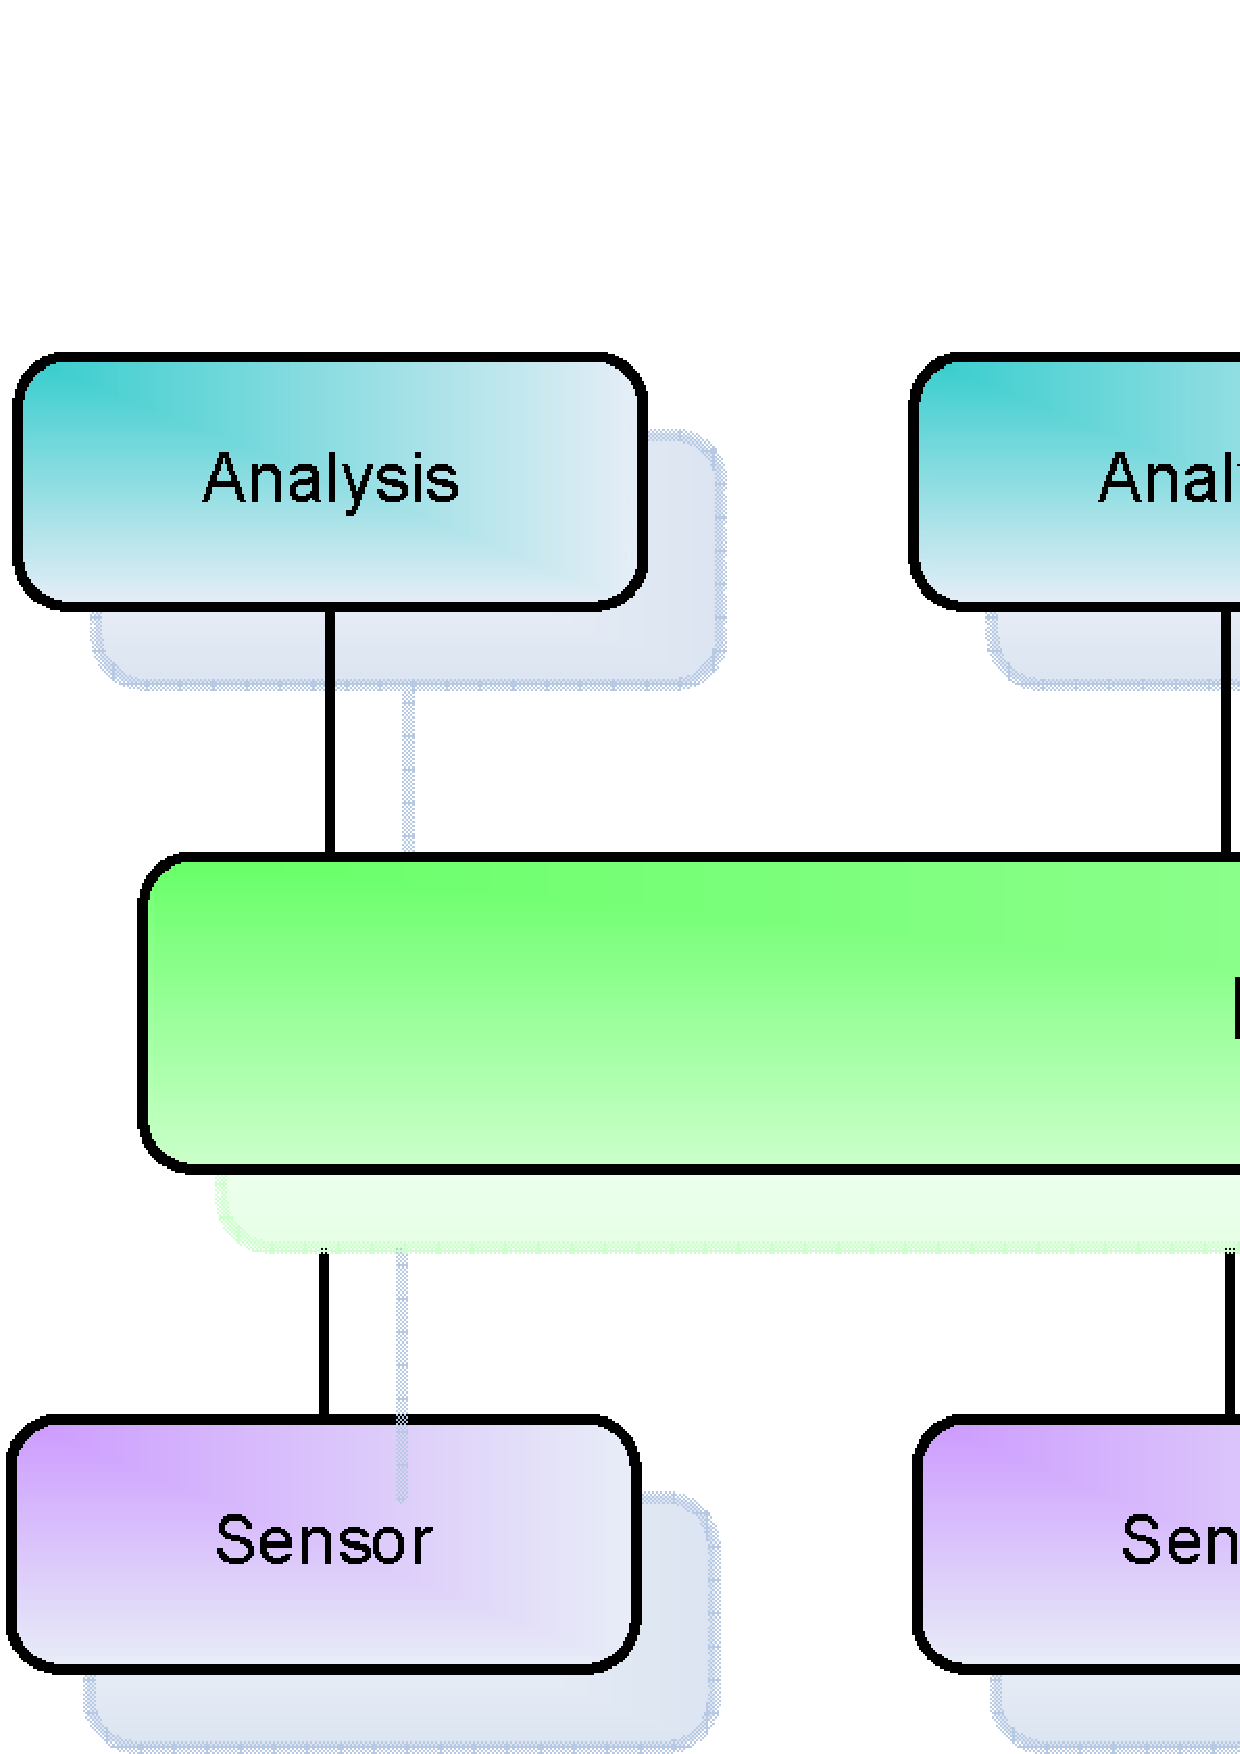
\includegraphics[width=1.00\textwidth ]{figures/HackystatMicroKernel}
  \caption{Hackystat Architecture - Internal View}
  \label{fig:HackystatMicroKernel}
\end{figure}




\subsection{Metrics Collection}

Sensors communicate with Hackystat server using SOAP through HTTP channels. As of this writing,  sensors are implemented for interactive development environments (such as Eclipse, Emacs, JBuilder, Vim, and Visual Studio), office productivity applications(such as Word, Excel, and Powerpoint), size measurement tools (such as CCCC and LOCC), testing tools (such as JUnit and JBlanket), configuration management tools (such as CVS and Harvest), and defect tracking tools (such as Jira). %{\em Build tools}, including Ant and the Unix command line;




\subsection{Project Management}  %Ref: CSDL TechReport 03-12

Metrics analyses are most useful on project level, which require information such as which developers are working together, what files they are collaboratively developing, and the time period during which a given increment of the system is under development.

Hackystat provides infrastructure for project level analysis through project definition. A project definition specifies the set of developers who are collaborating together, as well as the directory hierarchies containing the project files. The system sends the developers specified in this project definition an email indicating that they have been defined within a project. They must explicitly confirm their agreement to participate in this project definition, which implies their agreement to allow their metrics to be used in project-level analyses that will be visible to all project members.






\subsection{Analyses and Alerts}

Hackystat supports two styles of information retrieval: \textit{pull} and \textit{push}. Pull-style information retrieval is called ``analysis''. Developers log onto the Hackystat server and run analyses on their product and process metrics through a web interface. Push-style information retrieval is called ``alert''. Hackystat sends out automated email message when incoming metrics activate user-defined triggers. The message usually contains summary information, and a link which directs users to the Hackystat server for more detailed pull-style analysis.




%%%%%%%%%%%%%%%%%%%%%%%%%%%%%%%%%%%%%%%%%%%%%%%%%%%%%%%%%%%%%%%%%%%%%%%%%%%%%%
%%%%%%%%%%%%%%%%%%%%%%%%%%%%%%%%%%%%%%%%%%%%%%%%%%%%%%%%%%%%%%%%%%%%%%%%%%%%%%

\section{Software Project Telemetry Implementation}  \label{Implementation:Telemetry}


The reference implementation of software project telemetry is based on Hackystat.

\begin{figure}[tbp]
  \centering
  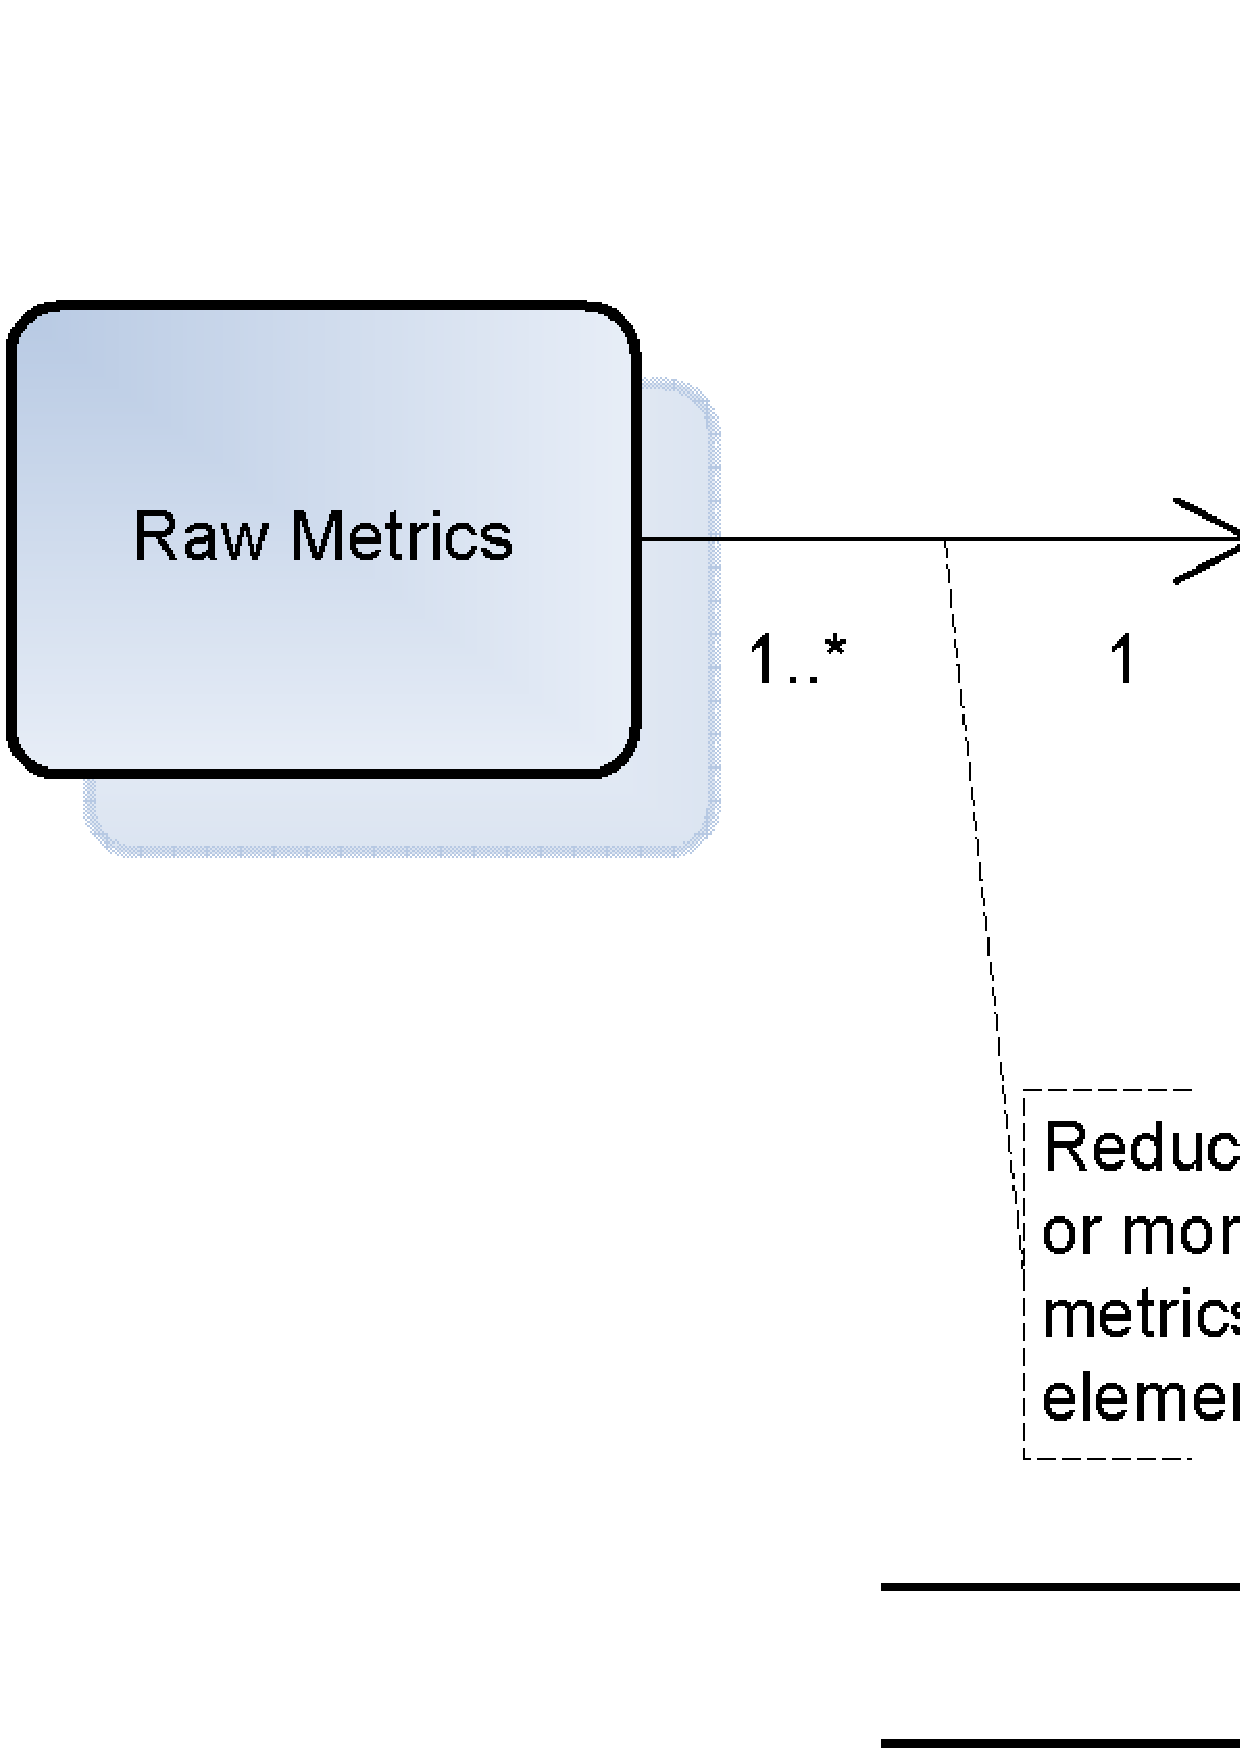
\includegraphics[width=1.00\textwidth ]{figures/TelemetryInternal}
  \caption{Telemetry Internals}
  \label{fig:TelemetryInternal}
\end{figure}

\begin{figure}[tbp]
  \centering
  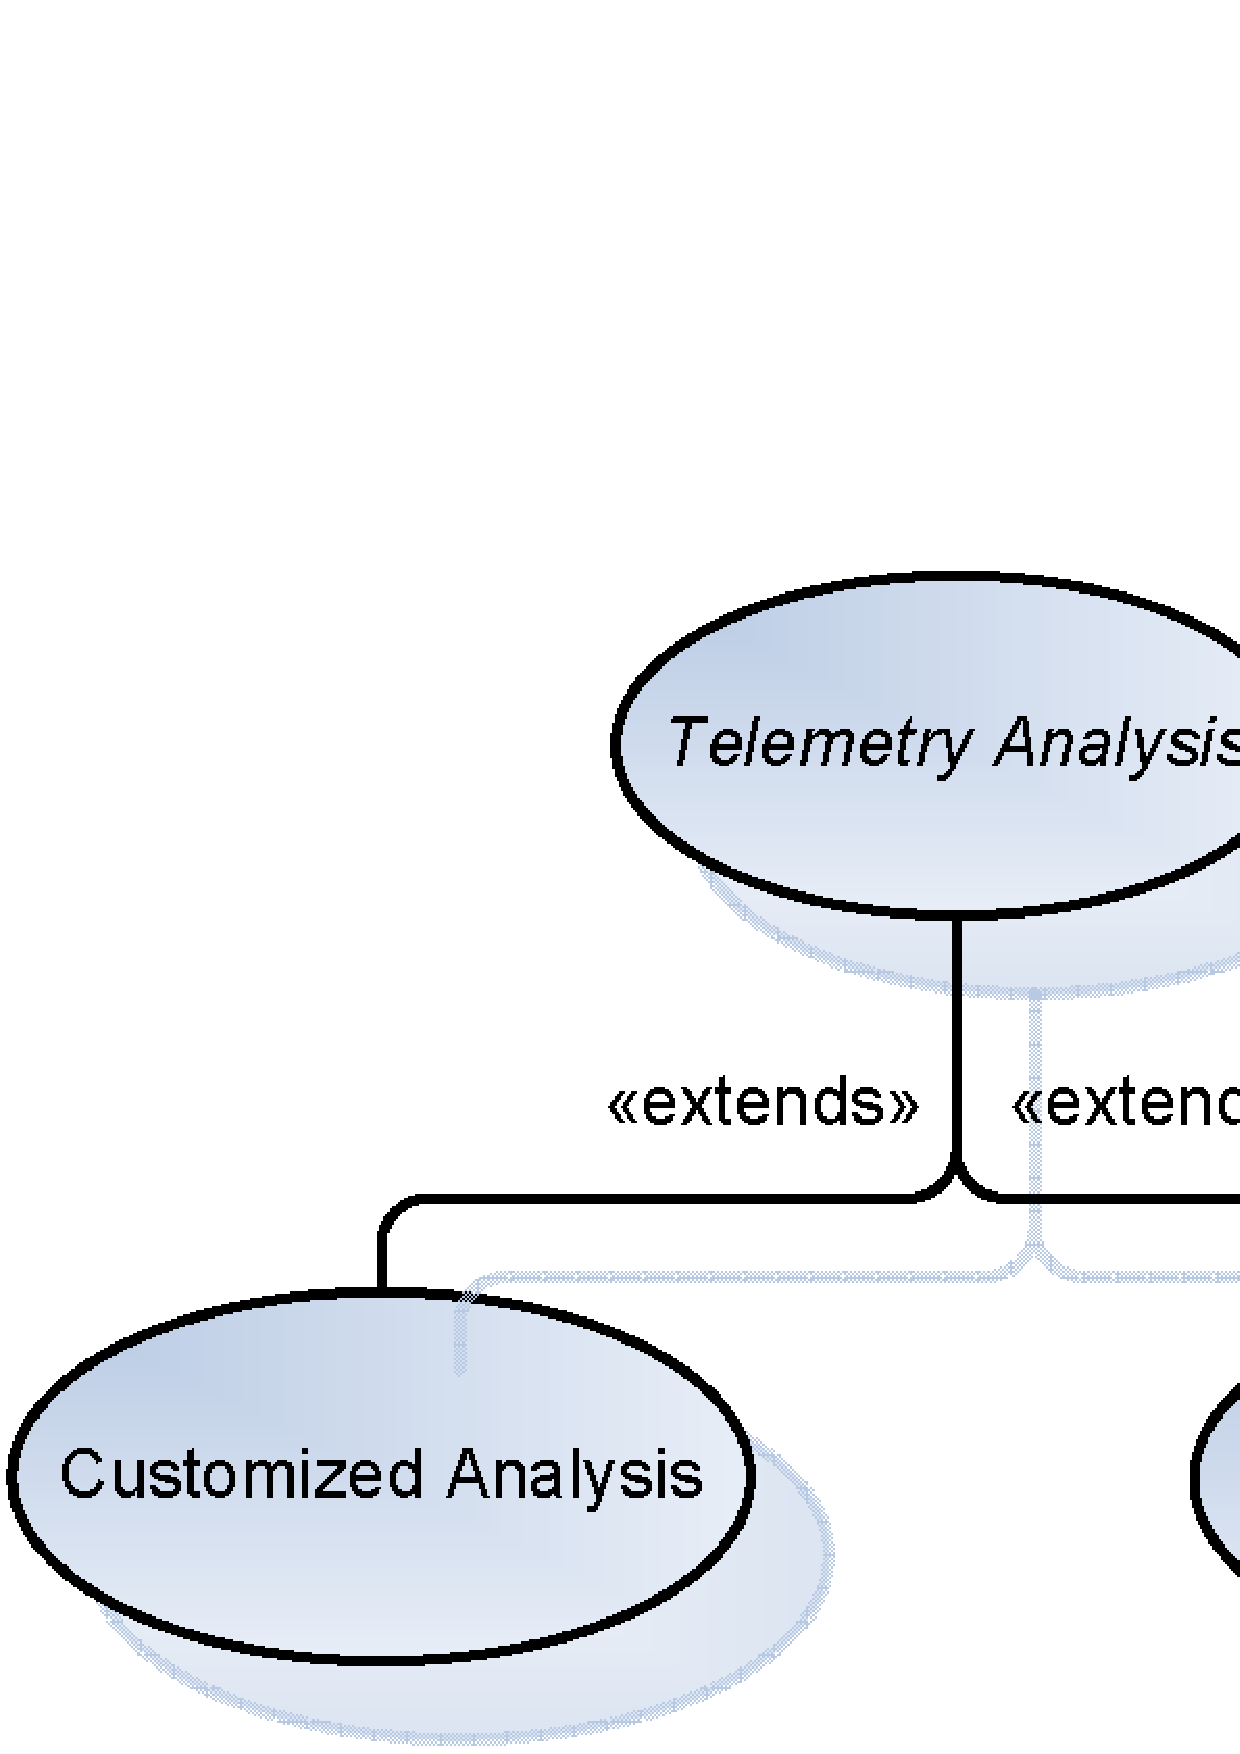
\includegraphics[width=1.00\textwidth]{figures/TelemetryExternal}
  \caption{Telemetry Externals}
  \label{fig:TelemetryExternal}
\end{figure}





\subsection{Telemetry Language Interpreter}

The telemetry language interpreter consists of 2 components: (1) the parser, and (2) the evaluator.

The parser is responsible for parsing user input into internal intermediate representation. 
[a chart show java objects]


The evaluator is responsible for evaluating the intermediate representation, and the final output is either a telemetry chart or a telemetry report. The evaluator simulates a stack-based computer. It turns the internal java object representation into post-fix format. Telemetry stream collections and numerical constants are push onto the stack. When an operand is encounter, they are popped off participating in the evaluation, and the result is again pushed onto the stack.

[a chart show how stack works].










\subsection{Telemetry Reducer Loading Mechanism}

%The implementation uses reducers to abstract raw sensor data (a.k.a. software metrics) to high level telemetry streams.

This reference implementation employs a dynamics mechanism to discover and load reducers at run time. 

Several reducers are supplied with this implementation:
\begin{itemize}
	\item 
\end{itemize}









\subsection{Telemetry Definition Management Console}














\subsection{Telemetry Analyses}

It includes:
\begin{itemize}
	\item Telemetry Chart Analysis
	\item Telemetry Report Analysis
	\item Telemetry Expert Analysis
\end{itemize}


Telemetry chart and report analysis generates telemetry chart or report respectively from pre-defined templates. User only needs to select a template from a drop down list and click a button. This is especially useful for novice users because it eliminates the need to learn Hackystat telemetry language which lowers adoption barrier of the technology. 

The expert-mode analysis is more flexibility. It allows user to specify directly what kind of report to generate in telemetry language. Figure \ref{fig:HackystatArchitecture} shows a screen shot of this analysis.

\begin{figure}[p]
  \centering
  
\includegraphics[height=0.90\textheight]{figures/TelemetryExpertAnalysis}
  \caption{Telemetry Export Analysis Screen Capture}
  \label{fig:TelemetryExpertAnalysis}
\end{figure}



\end{comment}





%While Hackystat and its telemetry subsystem (especially telemetry language) provide a flexible mechanism to generate telemetry streams, the capability is constrained by the raw metrics collected by Hackystat data collection infrastructure and the availability of reduction functions. (Reduction functions are responsible for generating elementary telemetry streams from raw metrics data. Since the management decision is based on telemetry streams, it is important to have the right telemetry streams or telemetry stream combination for the problem at hand. While Hackystat provides a flexible mechanism (telemetry language) to generate new telemetry streams, the streams that can be generated is constrained by the types of metrics collected by Hackystat. In other words, you can only generate telemetry streams based on collected metrics, or some combination of those metrics.
